\documentclass[a4paper,11pt]{ltjsarticle}
\usepackage{amsmath, mathtools, mathbbol, amssymb, bm, cancel, fancyhdr, anyfontsize, subcaption, multirow, wrapfig, graphicx, url, enumitem, ascmac, tikz, tikz-3dplot, makeidx}
\usepackage[luatex]{hyperref}
\usepackage[most]{tcolorbox}
\usepackage{ascolorbox}
\usepackage{stackengine}
\usepackage{cleveref}
\usepackage{appendix, adjustbox}

\hypersetup{
 pdfencoding=auto,
 setpagesize=false,
 bookmarksnumbered=true,
 bookmarksopen=true,
 colorlinks=true,
 linkcolor=blue,
 citecolor=blue,
 urlcolor=blue,
}

\crefname{equation}{式}{式}
\crefname{figure}{図}{図}
\crefname{table}{表}{表}

\crefname{section}{}{}
\creflabelformat{section}{#2#1節#3}
\crefname{subsection}{}{}
\creflabelformat{subsection}{#2#1節#3}

\newcommand{\crefpairconjunction}{と}
\newcommand{\crefrangeconjunction}{から}
\newcommand{\crefmiddleconjunction}{,}
\newcommand{\creflastconjunction}{,および}

\makeindex
\numberwithin{equation}{section}
\captionsetup{compatibility=false}
\usepackage[numbers]{natbib}
\usetikzlibrary{arrows, angles, quotes, cd}
\renewcommand{\cite}[1]{\textsuperscript{\citep{#1}}}
\newcommand{\idx}[1]{#1\index{#1}}
\newcommand{\Cancel}[2][black]{{\color{#1}\cancel{\color{black}#2}}}

\pagestyle{fancy}
\rhead{\textbf{\thepage}}
\cfoot{}
\renewcommand{\headrulewidth}{0pt}

\title{\textbf{モル計算と濃度計算}}
\author{ほうじ茶}
\date{\today}

\begin{document}

\maketitle

\begin{abstract}
  本稿では,モル計算と濃度計算を扱う.当然ながら,試薬の調整で必要な知識である.
  微生物を扱う上では,寒天培地をつくる際に\textbf{どのくらいの寒天が必要なのか?},植物の成分抽出をする上では,\textbf{エタノールの濃度はどのくらいが適切なのか?}などを考える必要がある.
  これらの計算ができない限り,実験系を組むことができず実験のスタートラインに立てない.そのため,計算できるようになることを目的とする.

  化学Chemistryの基本的な考え方は,\textbf{すべての物質は粒で構成されている}ということである.
  その粒の構造や運動を,\textbf{実験的に導かれ}帰納的に体系化されていることを忘れないで欲しい.
\end{abstract}

\tableofcontents

\vspace{12pt}

\begin{center}
  \textbf{\color{blue}青文字}をクリックすると,対応したページに遷移する.

  本稿の著作権は,\href{https://creativecommons.org/licenses/by-nc-sa/4.0}{CC BY-NC-SA 4.0}を適応する.
\end{center}

\cleardoublepage

\section{国際単位系International System of units\cite{units-1}}
\label{sec: si}

\textbf{科学Science}の世界では,測定や計算に\textbf{国際単位系}\footnote{Si単位系ともいう.}という国際的に統一された単位系を使用する.
この単位系を用いて\textbf{数値と単位の組}でデータを示す.この組のことを\textbf{物理量}Physical quantityという.
7つの\textbf{基本単位}を組み合わせて\textbf{組立単位}にすることで,さまざまな単位を作ることができる.
組立単位を知ることによって,求めたい単位に変える\textbf{単位換算}Unit conversionを行うことができるようになる.

\subsection{基本単位Basic units}
\label{sec: basic units}

基本単位は次の7つである.

\begin{table}[hbtp]
  \caption{基本単位}
  \label{tab: basic units}
  \centering
  \begin{tabular}{rll}
    \hline
    データの種類 & 英語 & 単位 \\
    \hline
    時間 & {\color{cyan}$t$}ime & [s] \\
    距離 & {\color{cyan}$r$}oute & [m] \\
    電流 & {\color{cyan}$I$}ntensity of current & [A] \\
    質量 & {\color{cyan}$m$}ass & [kg] \\
    絶対温度 & {\color{cyan}$T$}emperture & [K] \\
    物質量 & {\color{cyan}$n$}umber & [mol] \\
    光度 & Luminous {\color{cyan}$I$}ntensity & [cd] \\
    \hline
  \end{tabular}
\end{table}

モル計算や濃度計算においては,\textbf{質量}$m$\ [kg],\textbf{物質量}$n$\ [mol]のみ登場する.
質量は,単に\textbf{重さ}という認識だと考えている人も多いが,\textbf{モル質量}\ [g/mol]の形で計算をする.
モル質量とは,\colorbox{yellow}{1\ [mol]あたりの\textbf{質量}}のことである.各原子ごとに一義の値が経験則から計算されているため,
その値を使えばよい.

\subsection{物質量Amount of substance\cite{units-6}}

原子1粒同士を比較しても,非常に小さいため明確に重さの違いは分からない.しかし,何万,何億の粒を集めて比較すると,違いが分かるようになる.
かつては,炭素原子を基準として12\ [g]になるために必要な数である\colorbox{yellow}{$6.022 \times 10^{23}$個(アボカドロ数)}を1\ [mol]としていた.ただし,「炭素」依存での定義であり普遍性に欠ける.

ここでアボガドロ定数$N_A$を$6.022,140,76 \times 10^{23}$\ [/mol]と定義することで,単位の大きさを定めた.
簡単に言えば,原子や分子の粒を$N_A$個のことを1\ [mol]と置いた.この考えは,12個を1ダースと置くのと同じである.

また,物質量以外が何を基準として定義されているのかは,\cref{col: basic def}に記載した.

\subsection{接頭辞Prefix}
\label{sec: prefix}

接頭辞とは,基本単位よりも\textbf{大きい・小さいことを表す指標}のことである.
Si接尾辞では$\times 10^{\pm 30}$まで定まっているが,よく使われる$\times 10^{\pm 12}$までを紹介する.

\begin{table}[htbp]
  \caption{Si接頭辞}
  \label{tab: prefix}
  \centering
  \begin{tabular}{cccccc}
    \hline
    ($+$)接頭辞 & 英語 & 指数乗 & ($-$)接頭辞 & 英語 & 指数乗 \\
    \hline
    T & {\color{cyan}T}era & $\times 10^{12}$ & p & {\color{cyan}p}ico & $\times 10^{-12}$ \\
    G & {\color{cyan}G}iga & $\times 10^{9}$ & n & {\color{cyan}n}ano & $\times 10^{-9}$ \\
    M & {\color{cyan}M}ega & $\times 10^{6}$ & $\mu$ & micro & $\times 10^{-6}$ \\
    k & {\color{cyan}k}ilo & $\times 10^{3}$ & m & {\color{cyan}m}illi & $\times 10^{-3}$ \\
    h & {\color{cyan}h}ecto & $\times 10^{2}$ & c & {\color{cyan}c}enti & $\times 10^{-2}$ \\
    da & {\color{cyan}d}ec{\color{cyan}a} & $\times 10^{1}$ & d & {\color{cyan}d}eci & $\times 10^{-1}$ \\
    \hline
  \end{tabular}
\end{table}

マイナス乗は,プラス乗にすると\textbf{逆数}になる.例えば,$10^{-6}$は$\dfrac{1}{10^6}$である.
また,$10^{-6}$は$\mu$と置き換えられる.この考え方ができるようになると,単位換算が容易になる.

\subsection{単位換算Unit conversion}
\label{sec: convertion}

単位は,\textbf{定義に基づいて}組み立てることで新しい単位ができる.
基本的には,\textbf{同じ意味を持つもの同士を分母と分子に置き},{\color{cyan}\textbf{約分する}}ことで求めたい単位へと変える.
\cref{eq: uc-1}は,「\textbf{1日は何秒か?}」を求めたものである.恐らく,一度は計算したことがあるだろう.

\begin{equation}
  1\ [\mathrm{day}] = 1\ \Cancel[orange]{[\mathrm{day}]} \times \frac{24\ \Cancel[cyan]{[\mathrm{hr}]}}{1\ \Cancel[orange]{[\mathrm{day}]}} \times \frac{60\ \Cancel[magenta]{[\mathrm{min}]}}{1\ \Cancel[cyan]{[\mathrm{hr}]}} \times \frac{60\ [\mathrm{sec}]}{1\ \Cancel[magenta]{[\mathrm{min}]}} = 86,400\ [\mathrm{sec}] \label{eq: uc-1}
\end{equation}

単位換算を行う上で押さえるポイントは,最初の単位と\textbf{求めたい単位に注目し}
定義として\textbf{どの物理量同士が等しいか}考え約分する必要がある.
今回の場合,1\ [day] と 24\ [hr]は定義より等しいので,分母と分子に置くことで理論上約分でき1と同じ意味となる.

次に,\cref{sec: prefix}の接頭辞を用いた単位換算を扱う.一例として,[mL]を[L]に変える場合を考える.

\begin{equation}
  1,000\ [\mathrm{{\color{cyan}m}L}] = 1,000 \times {\color{cyan}10^{-3}}\ [\mathrm{L}] = 1\ [\mathrm{L}] \label{eq: uc-2}
\end{equation}

[mL]の{\color{cyan}m}は,\cref{tab: prefix}を参照すると指数乗は{\color{cyan}$10^{-3}$}である.
そのため,まず\textbf{接頭辞を指数乗に変える}.そのあと,指数乗を掛けることで単位を換算できる.

\clearpage

その他,戸惑いやすいが変換できるものを紹介する.

\begin{table}[htbp]
  \caption{単位変換}
  \label{tab: unit}
  \centering
  \begin{tabular}{rl}
    \hline
    体積と質量 & 1\ [cc] = 1\ [mL] = 1\ [g] \\
    体積と密度 & 1\ [L] := 1\ [dm$^3$] = 0.001\ [m$^3$] \\
    モル濃度 & 1\ [M] := 1\ [mol/L] \\
    \hline
  \end{tabular}
\end{table}

\href{https://example.com}{%
  \adjustbox{border=2pt solid blue}{%
    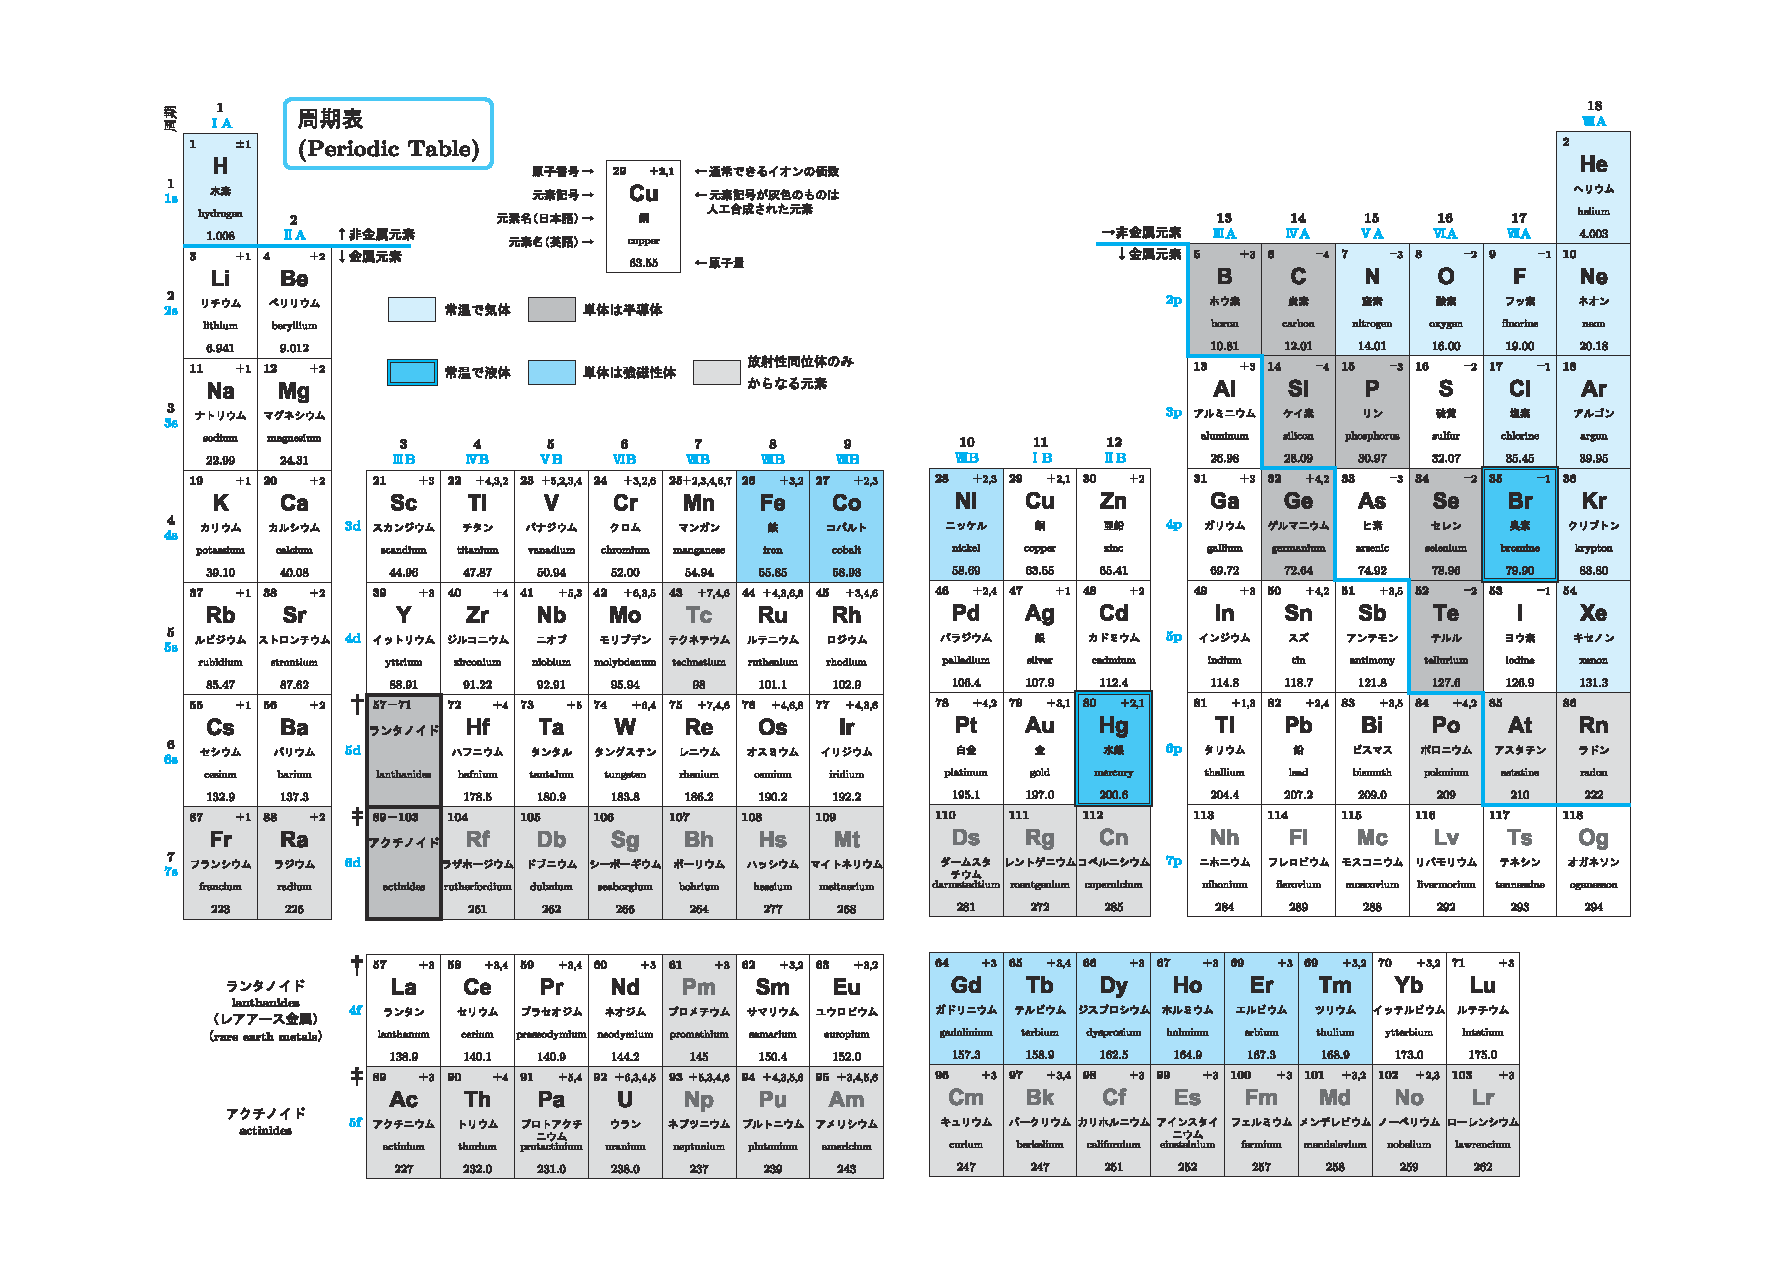
\includegraphics[width=0.5\textwidth]{periodic_table.pdf}%
  }%
}

\cleardoublepage

\lhead{}
\pagenumbering{alph}
\phantomsection
\addcontentsline{toc}{section}{参考文献}
\bibliographystyle{plain}
\bibliography{ref.bib}

\cleardoublepage
\appendix
\section{基本単位の定義\cite{units-1}}
\label{col: basic def}

\hspace{5pt}

基本単位には,\textbf{一義性}\footnote{ただ1つに定まる性質のこと.}と\textbf{普遍性}\footnote{広く全ての場合にあてはめることができる性質のこと.}を持った基準が必要であり世界共通のものである.
その\textbf{厳密な定義}を紹介する.

\subsection*{時間の定義\cite{units-2}}

原子や分子には,固有の振動数の光や電波を吸収し放射する性質がある.その性質を利用して,セシウム原子のマイクロ波の振動$\Delta \nu_{\mathrm{Cs}}$を,$9,192,631,770$回数えたときを1秒と定義した.
[Hz]\footnote{ヘルツは,\textbf{回数}を示す単位である.}は\textbf{単位時間あたりの振動数}のことであり,[/s]と同じ意味である.

\subsection*{距離の定義}

真空中の光の速さ$c$を$299,792,458$ [m/s]と定めることによって定義した.

\subsection*{電流の定義\cite{units-5}}

かつては,真空中に1\ [m]間隔で平行に置いた無限に長い2本の導体がそれぞれを流れ,これらの導体の長さ1\ [m]につき$2 \times 10^{-7}$\ [N]の力を及ぼし合う一定の電流を1\ [A]としていた.
ただし,電流の単位を力として定義している.これは\textbf{電流は素粒子の流れ}であるという本質が分かっていなかったためである.そのため,2019 年に改定された.

新たに電気素量$e$\footnote{ファラデー定数(電子1 [mol]が持つ電気量の値のこと)を$F$,アボガドロ定数を$N_A$とすると,$e=\tfrac{F}{N_A}$でも求められる.}を$1.602,176,634 \times 10^{−19}$ [C]と定めることによって定義した.
[C]は\textbf{単位時間あたりの電気量}のことであり,$\mathrm{[A \cdot s]}$と同じ意味である.

\subsection*{質量の定義\cite{units-3}}

かつては,国際キログラム原器(白金とイリジウムの合金で出来た円柱)の質量を1\ [kg]としていた.
ただし,経年劣化により一義性に欠けるため,電流と同様に2019年に改定された.
  
物体の静止質量を$m$,光子の周波数を$\nu$,プランク定数を$h$とすると,
アインシュタインの相対性理論と光量子仮説によれば\cref{eq: einstein}である.

  \begin{equation}
    E = mc^2 = h \nu \label{eq: einstein}
  \end{equation}

ここでプランク定数$h$を$6.626,070,15 \times 10^{−34}\ \mathrm{[J \cdot s]}$と定義することで,
周波数$\nu$\ [Hz]の光子のエネルギー$E$と等価な質量が$m$\ [kg]である.

\subsection*{絶対温度の定義\cite{units-4}}

かつては,氷と水,水蒸気が共存する温度$0.01 ^\circ \mathrm{C}$の約273分の1を1\ [K]としていた.
ただし,「水」という物質に依存しており,かつ三重点の実現可能性が低いため電流と同様に2019年に改定された.

理想気体の場合,個々の分子は他の分子と衝突するとき以外は自由に動く.
1個の単原子の平均の運動エネルギーは,質量を$m$,2乗平均速度を$\overline{v^2}$,ボルツマン定数$k$,絶対温度$T$とすると\cref{eq: boltzmann-1}である.

\begin{subequations}

  \begin{equation}
    \frac{1}{2} m \overline{v^2} = \frac{3}{2} kT \label{eq: boltzmann-1}
  \end{equation}

一方で,理想気体の分子$nN_A$個\footnote{$N_A$はアボガドロ定数であり,ボルツマン定数$k$と乗算することで気体定数$R$となる.}を体積$V$の容器に入れた場合,その圧力$p$は,質量$m$と2乗平均速度$\overline{v^2}$とすると\cref{eq: boltzmann-2}である.

  \begin{equation}
    p = \frac{1}{3} \frac{nN_Am}{V} \overline{v^2} \label{eq: boltzmann-2}
  \end{equation}

\cref{eq: boltzmann-1,eq: boltzmann-2}より,\cref{eq: air}の理想気体の状態方程式が得られる.

  \begin{equation}
    p(T)V = nN_AkT \label{eq: air}
  \end{equation}

\end{subequations}

エネルギーは$[\mathrm{J}] = [\mathrm{kg \cdot m^2/s^2}]$で表される.
ここでボルツマン定数$k$を$1.380, 649 \times 10^{−23}$\ [J/K]と定義することで,単位の大きさを定めることと同じになる.

\subsection*{光度の定義}

特定の周波数$540 \times 10^{12}$\ [Hz]の緑色の光を出す特定の方向に,放射強度$K_{\mathrm{cd}}$が683 [lm/W]である点光源の光度を,1\ [cd]と定義した.

\end{document}